\chapter{РЕАЛИЗАЦИЯ СИСТЕМЫ АВТОМАТИЗАЦИИ УПРАВЛЕНИЯ ЖИЗНЕННЫМ ЦИКЛОМ ВЕБ-СЕРВИСА}
\label{cha:impl}

\section{Подготовка GitLab}

Перед реализацией необходимо произвести базовую настройку окружения.
Для этого был зарегистрирован GitLab аккаунт, установле SSH ключ и создана группа проекта.
Результаты создания группы представлены на рисунке \ref{fig:group-ready}.

\begin{figure}[ht]
    \centering
    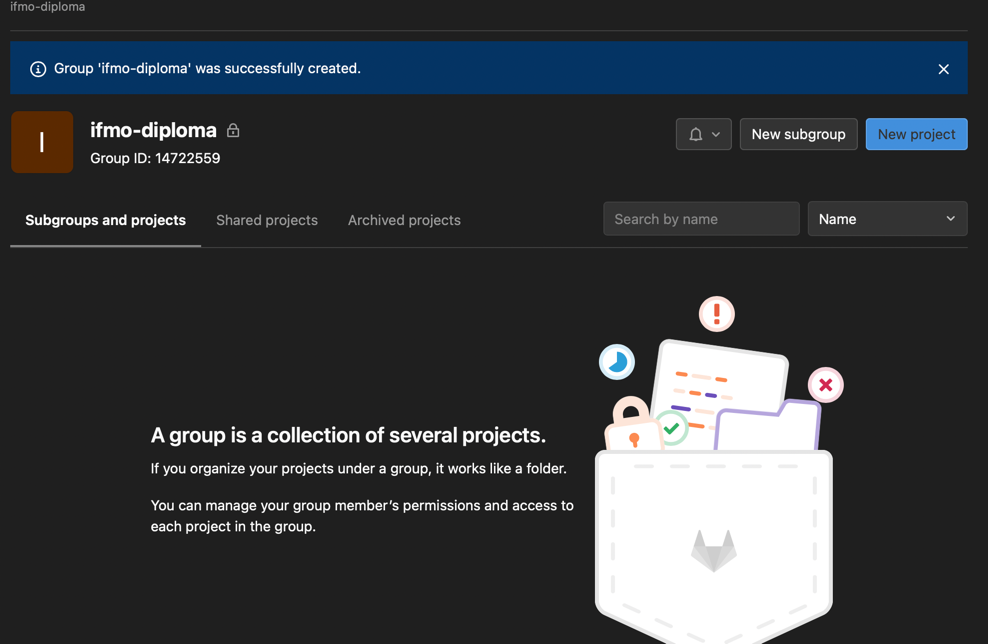
\includegraphics[scale=0.4]{figures/0}
    \caption{Скриншот создания группы в GitLab}
    \label{fig:group-ready}
\end{figure}

Следующим этапом было произведено создание необходимых репозиториев с последующей загрузкой исходного кода предоставленного для работы веб-сервиса:

\begin{itemize}
    \item web-client --- репозиторий для хранения исходного кода веб-клиента проекта,
    \item api --- репозиторий для хранения исходного кода API проекта.
    \item node packages --- репозиторий для хранения исходного кода общих npm зависимостей проекта.
\end{itemize}

Так же в корне каждого репозитория был загружен Dockerfile для развёртки данного сервиса.
Так как в качестве модели ветвления была выбрана модель git flow, то так же были подговлены соответствующие ветки в репозиториях под разные окружения: develop, testing и release.
Установка доступа к данным репозиториям предоставляется только соответсвующим разработчикам данных программных решений в целях безопасности.

Подготвка хранилищ npm пакетов и Docker образов не требуется, так как GitLab берёт на себя данную отвественность и не требует дополнительных действий от пользователя.

На следующем этапе был подготовлен репозиторий deployment для хранения общих скриптов и конфигураций окружения и развёртки.
Установка доступа к этому репозиторию предоставляется только команде обеспечения развёртки в целях безопасности.
Результаты создания репозиториев представлены на рисунке \ref{fig:reps-ready}.

\begin{figure}[ht]
    \centering
    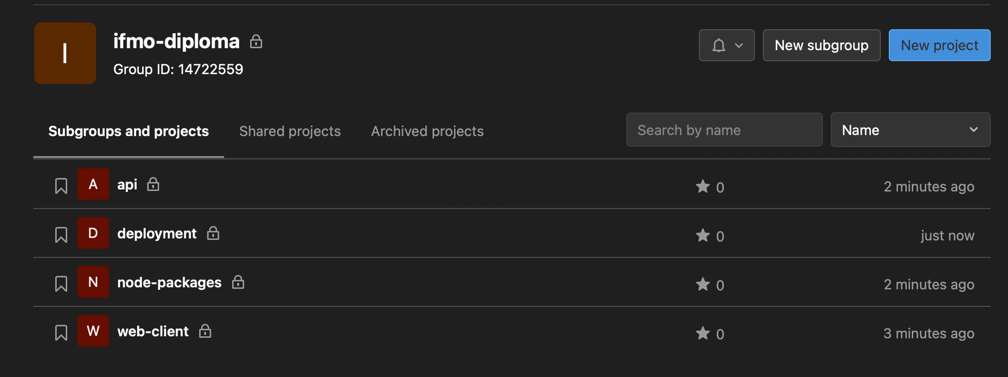
\includegraphics[scale=0.4]{figures/1}
    \caption{Скриншот создания репозиториев в GitLab}
    \label{fig:reps-ready}
\end{figure}

\section{Установка кластера Docker Swarm}

Следующим этапом был установлен и настроен Docker Swarm кластер.

Для этого на рабочей системе было произведено открытие необходимых портов в операционной системе\cite{linuxPocket}:
\begin{lstlisting}[language=bash,caption={Открытие портов в Linux}]
$ sudo ufw allow 2377
$ sudo ufw allow 7946
$ sudo ufw allow 4789
\end{lstlisting}

Дальше была произведена инициализация кластера на сервере:
\begin{lstlisting}[language=bash,caption={Инициализация кластера}]
$ docker swarm init --advertise-addr 192.168.1.101
  Swarm initialized: current node (dxn1zf6l61qsb1josjja83ngz) is now a manager.
  To add a worker to this swarm, run the following comman:
    docker swarm join --token <token> 192.168.1.101:2377
  To add a manager to this swarm, run 'docker swarm join-token manager' and follow the instructions.
\end{lstlisting}

В данном этапе нет необходимости при использовании Kubernetes.

\section{Установка и настройка GitLab Runner}

После была произведена установка и настройка GitLab Runner на рабочем сервере.
В качестве дистрибутива на этапе проектирования был выбран Docker, как самый быстрый и удобный.
После установки необходимо зарегистрировать GitLab Runner, для этого на странице настроек CI/CD группы в GitLab был получен регистрационный токен.
Конфигурация runner производится путём редактирования config.toml\cite{web:gitlab:docs} файла в соответствии с этапом проектирования, основными настройками являются являются:

\begin{itemize}
    \item Установка executor --- docker executor,
    \item Установка volumes --- /var/run/docker.sock\cite{web:docker:docs},
    \item Установка pull-policy --- if-not-present,
    \item Установка concurrent --- 3.
\end{itemize}

На данном этапе runner полностью готов к работе и ожидает входящих задач.

\section{Описание CI/CD конфигураций}

На следующем этапе необходимо подготовить общие для работы сервисов конфигурации запуска, которые будут храниться в репозитории deployment:

\begin{itemize}
    \item build.yaml --- набор универсальных задач, предназначенный для сборки Docker образа и последующей загрузки в  регистр контейнеров,
    \item publish.yaml --- набор универсальных задач, предназначенный для оповещения кластера о об обонвлении сервиса для загрузки новой версии,
    \item publish-api.yaml --- расширенная версия publish.yaml, содержащая дополнительные задачи для проведения миграция базы данных в случае необходимости,
    \item build-package.yaml --- набор задач для для отслеживания к какому конкретному сервису принадлежит npm пакет путём построения графа зависимостей на основании package.json файлов,
    \item publish-package.yaml --- набор задач для загрузки собранного npm пакета .
\end{itemize}

Далее была произведена конфигурация на уровне сервисов компонентов, в репозитории api и web-client были добавлены конфигурации CI/CD путёт создания .gitlab-ci.yml файла, содержащие основные задачи.

Аналогичные задачи были описаны для репозитория node packages.

\section{Развёртка сервисов внутри кластера}

Завершающим этапом реализации является описание конфигурационных файлов Docker Swarm.
Для этого в настройках CI/CD репозитория deployment были добавлены переменные окружения (секреты) на все рабочие окружния (develop, testing и release),
содержащие аргументы сервисов компонентов системы (доступы к базе данных, секрет ключа авторизации и так далее)\cite{kuberForDevOps}.
Аналогично были добавлены Docker Swarm конфигурационные файлы под каждый окружения:

\begin{itemize}
    \item develop --- каждый сервис запускается на сервере в одном экзмепляре, ресурсы сервера сильно ограничены во избежание лишней нагрузки,
    \item testing --- аналогичен develop, только используется для целей ручного тестирования веб-сервиса,
    \item release --- web-client запускается в одном экзмепляре, база данных и api запускаются в трёх, большая часть ресурса отведена под эти сервисы.
\end{itemize}

%%% Local Variables:
%%% mode: latex
%%% TeX-master: "rpz"
%%% End:
